\documentclass[11pt]{amsbook}
\usepackage[utf8]{inputenc}
\usepackage[utf8]{inputenc}
\usepackage{Ceyhun}
\usepackage{amsTurkish}
\usepackage[turkish]{babel}
\usepackage{lipsum}

\begin{document}
\hPage{175}
çizge düzleme çizilemez' diye verebiliriz. Şekil 4.1.3 de de açıklandığı gibi, güney kutup özek ve kuzey kutup sonsuz alınarak, yuvarlağın düzlem üzerine izdüsümün yapılabileceğini biliyoruz.
Öyleyse, düzleme çizilebilen her çizgenin, yuvarlağa da çizilebileceğini söyleyebiliriz.
\begin{center}
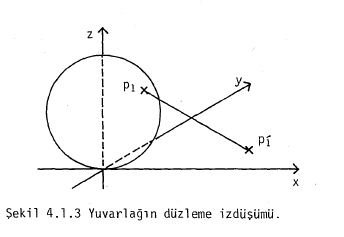
\includegraphics{images/figure-1}
\end{center}

\textbf{Tanım} 4.1.1 \begin{center}
Ayrıtları düğümlerden baska hiçbir\\
yerde kesismeden, yuvarlağa\\
çizilebilen çizgelere \underline{\textit{düzlemsel çizge}} \\denir.
\end{center}


Bu tanımdan, Şekil 4.1.1 deki çizgenin düzlemsel olduğu anlaşılır. Düzleme çizilemeyen çizgelere, \underline{\textit{düzlemsel olmayan çizge}} diyeceğiz. Düzlemsel bir çizgede, ayrıtların düzlem üzerinde tanımladığı kapalı bölgelere çizgenin \underline{\textit{içyüzleri}}, çizgenin

\end{document}
